%\subsection{Ejercicio 2}\label{subsec:ej2}

Para que la página esté en horizontal (apaisada) se usa la siguiente instrucción:

\begin{lstlisting}[language=PostScript, caption=Instrucción para página en horizontal, captionpos=b, label=fun:pghorizontal]
<< /PageSize [842 595] >> setpagedevice 
\end{lstlisting}

Para usar distintas tipografías antes del texto se define el tipo de fuente y el tamaño. Por ejemplo:
\begin{lstlisting}[language=PostScript, caption=Tipografía para título, captionpos=b, label=fun:tipografia1]
/Times-Roman findfont % Fuente
25 scalefont % Escala
setfont % Establecer como la fuente actual
\end{lstlisting}
Este es el formato para el texto \textit{PDIH} e \textit{Ines Ruiz}. Para que \textit{Ingeniera Informática} aparezca en cursiva hay que usar la orden:
\begin{lstlisting}[language=PostScript, caption=Tipografía en cursiva, captionpos=b, label=fun:tipografia2]
/Times-Italic findfont 14 scalefont setfont
\end{lstlisting}

Además, a la izquierda se ha dibujado un círculo con el comando \textit{arc}.
\begin{lstlisting}[language=PostScript, caption=Círculo de la tarjeta, captionpos=b, label=fun:circulo]
newpath % Círculo
    0.7 setgray % color gris claro
    3 setlinewidth
    200 300 80 0 360 arc   
    fill
stroke

newpath % Circunferencia
    0.3 setgray % color gris oscuro
    3 setlinewidth
    200 300 80 0 360 arc  
stroke
\end{lstlisting}
Para hacer el efecto de que el borde sea más oscuro que el relleno se han dibujado dos círculos con distintos tonos de grises. En el circulo interno se ha usado la instrucción \textit{fill} para indicar que la figura esté rellena.

A continuación se muestra la imagen obtenida\myref{fig:2ejer2}:
\begin{figure}[H]
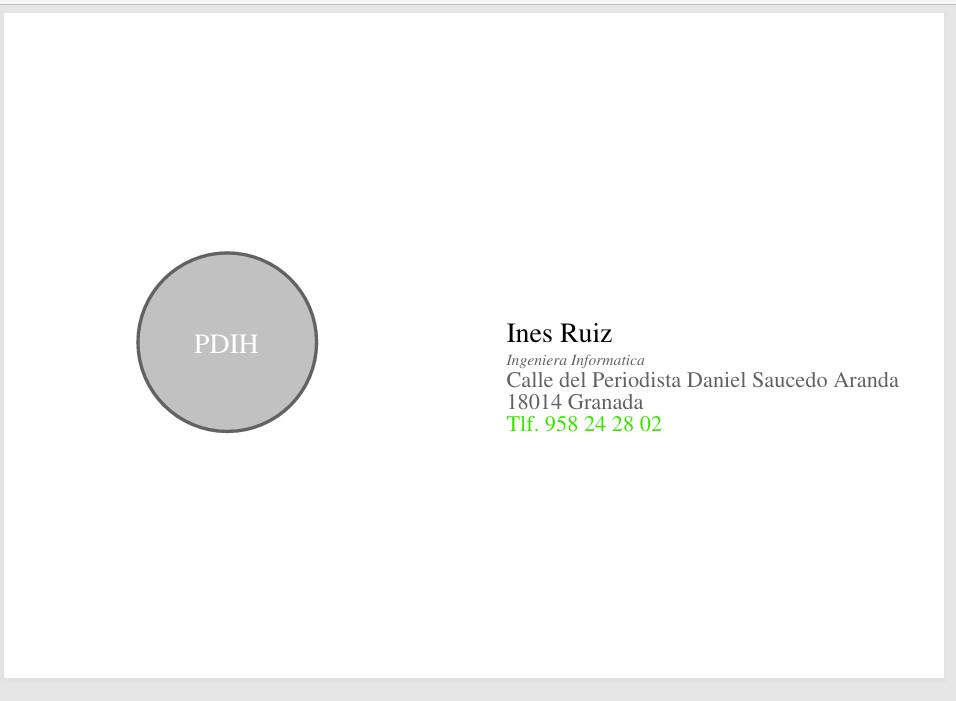
\includegraphics[width=0.9\textwidth]{images/ejer2.jpg}
\caption{Propuesta ejercicio 2}
\label{fig:2ejer2}
\end{figure}

El código completo se puede ver en el anexo \ref{anexo:ej2}. En el anexo \ref{anexo:pdf2} se puede ver la página pdf generada.